\newpage
\section*{Đề bài}
\addcontentsline{toc}{section}{Đề bài}

\par Dựa vào lý thuyết ``Chương 1 - Overview of Data Analytics and Descriptive Statistics'' đã học, ta biết được cách tính toán các chỉ số central tendency (mean, mode, median, quartiles), và dispersion (variance, standard deviation, range, standard error of mean, skewness, và kurtosis).

Mỗi sinh viên hãy thực hiện các yêu cầu bên dưới như sau:

\textbf{\underline{Yêu cầu:}}

\subsection*{Phần A: Dùng công cụ Excel, SPSS, Python và R tính toán.}

- Có file dữ liệu cổ phiếu VNG (mã VNZ, UpCom) đính kèm.

- Phân tích và tính toán các chỉ số thống kê mô tả ở trên cho cột ``Total Value'' trong file.

- Trực quan bằng Box Plot và Histogram của phân phối dữ liệu cột ``Total Value''.

\subsection*{Phần B: Phân tích thống kê mô tả từng bước (bằng tay, bút mực) dựa vào các công thức đã học ở Chương 1.}

\begin{figure}[!htp]
    \centering
    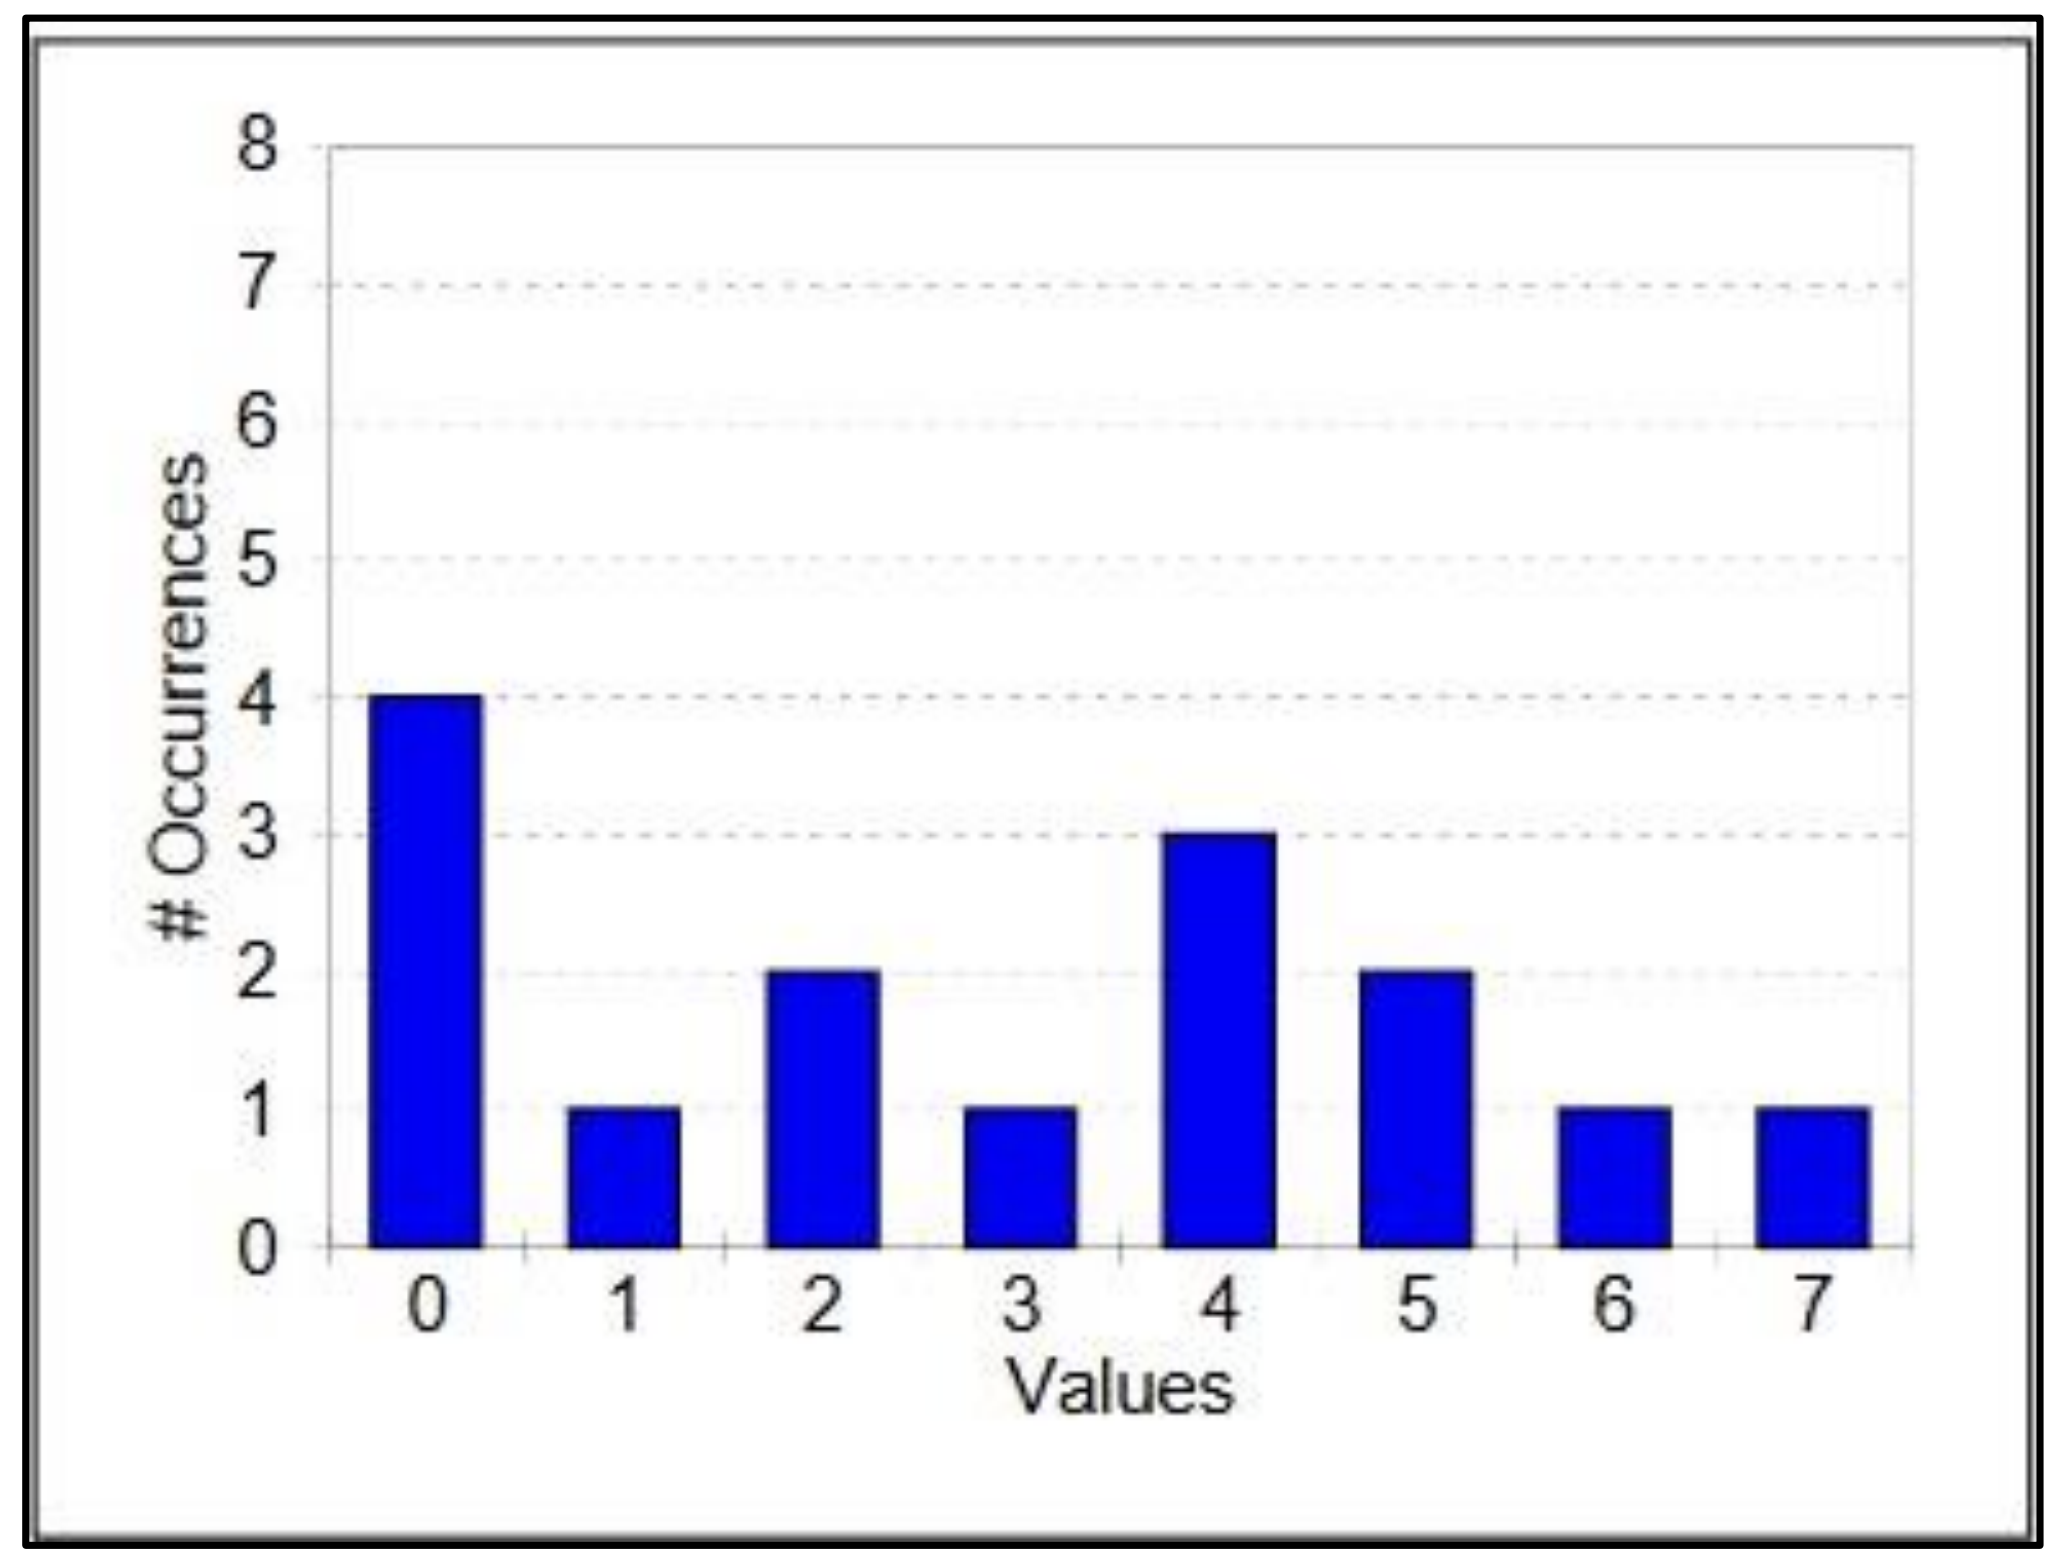
\includegraphics[width=0.6\textwidth]{LAB01/pics/YCDB.png}%
    \caption{Biểu đồ tần số (Hình P).}
    \label{fig:freq}
\end{figure}

Giả sử có hình \ref{fig:freq}, hãy xác định tập dữ liệu, phân tích và tính toán các chỉ số thống kê mô tả ở trên.

\textbf{Chú ý:}
\begin{itemize}
    \item Kết quả phần (A) và (B) phải được tóm tắt và chụp hình đưa vào tệp tin có quy cách đặt tên như sau: \texttt{MSSV\_Họtên\_Lab01\_Output.docx} (\texttt{.pdf}).
    \item Gửi đính kèm các file Excel, SPSS, R và Python của Phần A. Tương tự, quy cách đặt tên file như sau:
    \begin{itemize}
        \item \texttt{MSSV\_Họtên\_Lab01\_Excel.xlsx}
        \item \texttt{MSSV\_Họtên\_Lab01\_SPSS.sav} (và \texttt{.spv})
        \item \texttt{MSSV\_Họtên\_Lab01\_Python.ipynb}
        \item \texttt{MSSV\_Họtên\_Lab01\_R.r}
    \end{itemize}
    \item Đóng gói lại thành 01 tập tin duy nhất và nộp file này theo đúng deadline với quy cách đặt tên file như sau: \texttt{MSSV\_Họtên\_Lab01.rar} (.zip).
\end{itemize}


% Bắt đầu